
\documentclass[letterpaper,hide notes,xcolor={table,svgnames},pdftex]{beamer}
\def\showexamples{t}


%\usepackage[svgnames]{xcolor}

%% Demo talk
%\documentclass[letterpaper,notes=show]{beamer}

\usecolortheme{crane}%seahorse crane
\setbeamertemplate{navigation symbols}{}

\usetheme{MyPittsburgh}
%\usetheme{Frankfurt}

%\usepackage{tipa}

\usepackage{hyperref}
\usepackage{graphicx,xspace}
\usepackage[normalem]{ulem}

\newcommand\SF[1]{$\bigstar$\footnote{SF: #1}}

\usepackage{paratype}
\renewcommand*\familydefault{\sfdefault} %% Only if the base font of the document is to be sans serif
\usepackage[zerostyle=c]{newtxtt}
\usepackage[T1]{fontenc}

\newcounter{tmpnumSlide}
\newcounter{tmpnumNote}

\usepackage{xcolor}
\usepackage{tabu}
\definecolor{light-gray}{gray}{0.75}
\taburulecolor{light-gray}

% old question code
%\newcommand\question[1]{{$\bigstar$ \small \onlySlide{2}{#1}}}
% \newcommand\nquestion[1]{\ifdefined \presentationonly \textcircled{?} \fi \note{\par{\Large \textbf{?}} #1}}
% \newcommand\nanswer[1]{\note{\par{\Large \textbf{A}} #1}}


 \newcommand\mnote[1]{%
   \addtocounter{tmpnumSlide}{1}
   \ifdefined\showcues {~\tiny\fbox{\arabic{tmpnumSlide}}}\fi
   \note{\setlength{\parskip}{1ex}\addtocounter{tmpnumNote}{1}\textbf{\Large \arabic{tmpnumNote}:} {#1\par}}}

\newcommand\mmnote[1]{\note{\setlength{\parskip}{1ex}#1\par}}

%\newcommand\mnote[2][]{\ifdefined\handoutwithnotes {~\tiny\fbox{#1}}\fi
% \note{\setlength{\parskip}{1ex}\textbf{\Large #1:} #2\par}}

%\newcommand\mnote[2][]{{\tiny\fbox{#1}} \note{\setlength{\parskip}{1ex}\textbf{\Large #1:} #2\par}}

\newcommand\mquestion[2]{{~\color{red}\fbox{?}}\note{\setlength{\parskip}{1ex}\par{\Large \textbf{?}} #1} \note{\setlength{\parskip}{1ex}\par{\Large \textbf{A}} #2\par}\ifdefined \presentationonly \pause \fi}

\newcommand\blackboard[1]{%
\ifdefined   \showblackboard
  {#1}
  \else {\begin{center} \fbox{\colorbox{blue!30}{%
         \begin{minipage}{.95\linewidth}%
           \hspace{\stretch{1}} Some space intentionally left blank; done at the blackboard.%
         \end{minipage}}}\end{center}}%
         \fi%
}



%\newcommand\q{\tikz \node[thick,color=black,shape=circle]{?};}
%\newcommand\q{\ifdefined \presentationonly \textcircled{?} \fi}

\usepackage{listings}
\lstset{%
  keywordstyle=\bfseries,
  aboveskip=15pt,
  belowskip=15pt,
  captionpos=b,
  identifierstyle=\ttfamily,
  escapeinside={(*@}{@*)},
  stringstyle=\ttfamiliy,
  frame=lines,
  numbers=left, basicstyle=\scriptsize, numberstyle=\tiny, stepnumber=0, numbersep=2pt}

\usepackage{siunitx}
\newcommand\sius[1]{\num[group-separator = {,}]{#1}\si{\micro\second}}
\newcommand\sims[1]{\num[group-separator = {,}]{#1}\si{\milli\second}}
\newcommand\sins[1]{\num[group-separator = {,}]{#1}\si{\nano\second}}
\sisetup{group-separator = {,}, group-digits = true}

%% -------------------- tikz --------------------
\usepackage{tikz}
\usetikzlibrary{positioning}
\usetikzlibrary{arrows,backgrounds,automata,decorations.shapes,decorations.pathmorphing,decorations.markings,decorations.text}

\tikzstyle{place}=[circle,draw=blue!50,fill=blue!20,thick, inner sep=0pt,minimum size=6mm]
\tikzstyle{transition}=[rectangle,draw=black!50,fill=black!20,thick, inner sep=0pt,minimum size=4mm]

\tikzstyle{block}=[rectangle,draw=black, thick, inner sep=5pt]
\tikzstyle{bullet}=[circle,draw=black, fill=black, thin, inner sep=2pt]

\tikzstyle{pre}=[<-,shorten <=1pt,>=stealth',semithick]
\tikzstyle{post}=[->,shorten >=1pt,>=stealth',semithick]
\tikzstyle{bi}=[<->,shorten >=1pt,shorten <=1pt, >=stealth',semithick]

\tikzstyle{mut}=[-,>=stealth',semithick]

\tikzstyle{treereset}=[dashed,->, shorten >=1pt,>=stealth',thin]

\usepackage{ifmtarg}
\usepackage{xifthen}
\makeatletter
% new counter to now which frame it is within the sequence
\newcounter{multiframecounter}
% initialize buffer for previously used frame title
\gdef\lastframetitle{\textit{undefined}}
% new environment for a multi-frame
\newenvironment{multiframe}[1][]{%
\ifthenelse{\isempty{#1}}{%
% if no frame title was set via optional parameter,
% only increase sequence counter by 1
\addtocounter{multiframecounter}{1}%
}{%
% new frame title has been provided, thus
% reset sequence counter to 1 and buffer frame title for later use
\setcounter{multiframecounter}{1}%
\gdef\lastframetitle{#1}%
}%
% start conventional frame environment and
% automatically set frame title followed by sequence counter
\begin{frame}%
\frametitle{\lastframetitle~{\normalfont(\arabic{multiframecounter})}}%
}{%
\end{frame}%
}
\makeatother

\makeatletter
\newdimen\tu@tmpa%
\newdimen\ydiffl%
\newdimen\xdiffl%
\newcommand\ydiff[2]{%
    \coordinate (tmpnamea) at (#1);%
    \coordinate (tmpnameb) at (#2);%
    \pgfextracty{\tu@tmpa}{\pgfpointanchor{tmpnamea}{center}}%
    \pgfextracty{\ydiffl}{\pgfpointanchor{tmpnameb}{center}}%
    \advance\ydiffl by -\tu@tmpa%
}
\newcommand\xdiff[2]{%
    \coordinate (tmpnamea) at (#1);%
    \coordinate (tmpnameb) at (#2);%
    \pgfextractx{\tu@tmpa}{\pgfpointanchor{tmpnamea}{center}}%
    \pgfextractx{\xdiffl}{\pgfpointanchor{tmpnameb}{center}}%
    \advance\xdiffl by -\tu@tmpa%
}
\makeatother
\newcommand{\copyrightbox}[3][r]{%
\begin{tikzpicture}%
\node[inner sep=0pt,minimum size=2em](ciimage){#2};
\usefont{OT1}{phv}{n}{n}\fontsize{4}{4}\selectfont
\ydiff{ciimage.south}{ciimage.north}
\xdiff{ciimage.west}{ciimage.east}
\ifthenelse{\equal{#1}{r}}{%
\node[inner sep=0pt,right=1ex of ciimage.south east,anchor=north west,rotate=90]%
{\raggedleft\color{black!50}\parbox{\the\ydiffl}{\raggedright{}#3}};%
}{%
\ifthenelse{\equal{#1}{l}}{%
\node[inner sep=0pt,right=1ex of ciimage.south west,anchor=south west,rotate=90]%
{\raggedleft\color{black!50}\parbox{\the\ydiffl}{\raggedright{}#3}};%
}{%
\node[inner sep=0pt,below=1ex of ciimage.south west,anchor=north west]%
{\raggedleft\color{black!50}\parbox{\the\xdiffl}{\raggedright{}#3}};%
}
}
\end{tikzpicture}
}


%% --------------------

%\usepackage[excludeor]{everyhook}
%\PushPreHook{par}{\setbox0=\lastbox\llap{MUH}}\box0}

%\vspace*{\stretch{1}

%\setbox0=\lastbox \llap{\textbullet\enskip}\box0}

\setlength{\parskip}{\fill}

\newcommand\noskips{\setlength{\parskip}{1ex}}
\newcommand\doskips{\setlength{\parskip}{\fill}}

\newcommand\xx{\par\vspace*{\stretch{1}}\par}
\newcommand\xxs{\par\vspace*{2ex}\par}
\newcommand\tuple[1]{\langle #1 \rangle}
\newcommand\code[1]{{\sf \footnotesize #1}}
\newcommand\ex[1]{\uline{Example:} \ifdefined \presentationonly \pause \fi
  \ifdefined\showexamples#1\xspace\else{\uline{\hspace*{2cm}}}\fi}

\newcommand\ceil[1]{\lceil #1 \rceil}


\AtBeginSection[]
{
   \begin{frame}
       \frametitle{Outline}
       \tableofcontents[currentsection]
   \end{frame}
}



\pgfdeclarelayer{edgelayer}
\pgfdeclarelayer{nodelayer}
\pgfsetlayers{edgelayer,nodelayer,main}

\tikzstyle{none}=[inner sep=0pt]
\tikzstyle{rn}=[circle,fill=Red,draw=Black,line width=0.8 pt]
\tikzstyle{gn}=[circle,fill=Lime,draw=Black,line width=0.8 pt]
\tikzstyle{yn}=[circle,fill=Yellow,draw=Black,line width=0.8 pt]
\tikzstyle{empty}=[circle,fill=White,draw=Black]
\tikzstyle{bw} = [rectangle, draw, fill=blue!20, 
    text width=4em, text centered, rounded corners, minimum height=2em]
    
    \newcommand{\CcNote}[1]{% longname
	This work is licensed under the \textit{Creative Commons #1 3.0 License}.%
}
\newcommand{\CcImageBy}[1]{%
	\includegraphics[scale=#1]{creative_commons/cc_by_30.pdf}%
}
\newcommand{\CcImageSa}[1]{%
	\includegraphics[scale=#1]{creative_commons/cc_sa_30.pdf}%
}
\newcommand{\CcImageNc}[1]{%
	\includegraphics[scale=#1]{creative_commons/cc_nc_30.pdf}%
}
\newcommand{\CcGroupBySa}[2]{% zoom, gap
	\CcImageBy{#1}\hspace*{#2}\CcImageNc{#1}\hspace*{#2}\CcImageSa{#1}%
}
\newcommand{\CcLongnameByNcSa}{Attribution-NonCommercial-ShareAlike}


\newenvironment{changemargin}[1]{% 
  \begin{list}{}{% 
    \setlength{\topsep}{0pt}% 
    \setlength{\leftmargin}{#1}% 
    \setlength{\rightmargin}{1em}
    \setlength{\listparindent}{\parindent}% 
    \setlength{\itemindent}{\parindent}% 
    \setlength{\parsep}{\parskip}% 
  }% 
  \item[]}{\end{list}} 




\title{Lecture 23 --- Advanced Arrays }

\author{J. Zarnett\\
\texttt{jzarnett@uwaterloo.ca}}
\institute{Department of Electrical and Computer Engineering \\
  University of Waterloo}
\date{\today}

\begin{document}

\begin{frame}
  \titlepage
  
  \begin{center}
  \small{Acknowledgments: W.D. Bishop}
  \end{center}
\end{frame}


\begin{frame}
\frametitle{Arrays in Memory}
Now that we are familiar with pointers and some basics about memory organization, we can return to the subject of arrays.

It is important to remember the difference between a value type and a pointer type when working with arrays:\\
\begin{itemize}
	\item An array of value types provides storage for values;\\
	\item An array of pointer types provides storage for pointers.
\end{itemize}

This has an important implication:
A declaration of an array of structure pointers, for example, does not provide storage for fields.

\end{frame}

\begin{frame}[fragile]
\frametitle{Reference Type Array Example}

Consider an array of Student entries where each \texttt{Student} object has a name member field and an age member field:

{\scriptsize
\begin{verbatim}
struct Student[5] list;	// Declare an array of references to student structs
	
// At this point, list[0], list[1], list[2], 
// list[3], and list[4] are null references

list[0].name = "Bill";
list[0].age = 18;
list[1].name = "Bonnie";
list[1].age = 21;
list[2].name = "Dave";
list[2].age = 20;
list[3].name = "Austin";
list[3].age = 19;
list[4].name = "Kris";
list[4].age = 20;
\end{verbatim}
}
Notice that creating the array was not enough.\\
\quad We also had to populate the structures.

\end{frame}

\begin{frame}
\frametitle{Reference Type Array Example}

And here's what that code will produce in memory:

\begin{center}
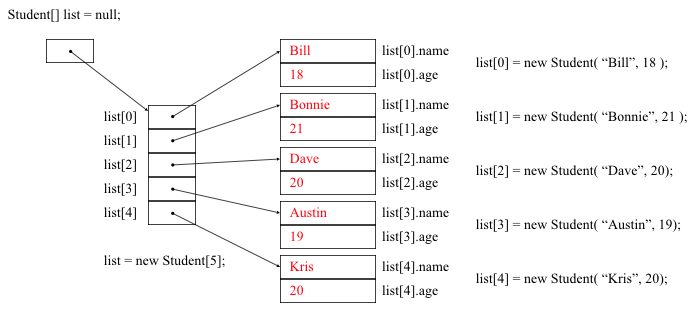
\includegraphics[width=\textwidth]{images/students.png}
\end{center}

Note that there are six references defined in total.

\end{frame}



\begin{frame}
\frametitle{Regular Arrays}
Remember earlier in the term our examination of arrays included multidimensional arrays.

\texttt{int[][] jag;}\\
\quad Declares this in a single array.

\end{frame}



\begin{frame}
\frametitle{Array Storage}
Internally, C++ stores arrays using row-major order.

Suppose we ask for an integer array of 3$\times$3: \texttt{int[3][3]}.

A 3$\times$3 array of integers  stored in contiguous memory locations:

\begin{center}
	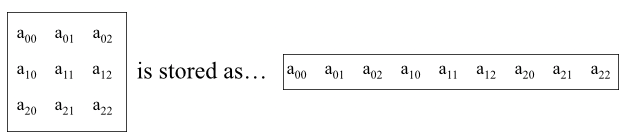
\includegraphics[width=\textwidth]{images/rowmajor.png}
\end{center}

\end{frame}

\begin{frame}[fragile]
\frametitle{Less Contiguous Array Storage}
Let's contrast that against an array declared as follows:\\

\begin{verbatim}
int n = 5;
int m = 7
int* array = new int[n];

for( int i = 0; i < n; ++i )
{
    array[i] = new int[m];
}
\end{verbatim}

What does this look like in memory?

\end{frame}

\begin{frame}
\frametitle{Jagged Array in Memory}

Each of the arrays is allocated somewhere on the heap, but it could be anywhere in that relatively large area.

\begin{center}
	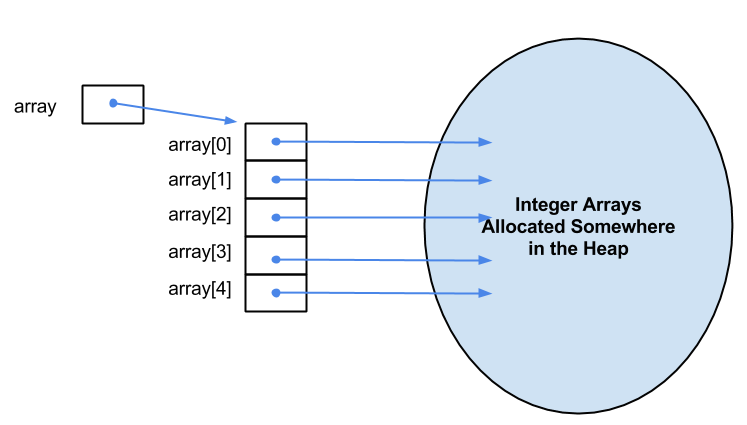
\includegraphics[width=0.85\textwidth]{images/jaggedArrayMemory.png}
\end{center}

(The first level of the array is also allocated somewhere on the heap).


\end{frame}

\begin{frame}
\frametitle{Jagged Arrays}

Arrays declared the first way have nicer syntax and are compact in memory.

Being compact in memory is advantageous because you can do pointer arithmetic to move around within the array.

It is also advantageous because of how CPUs work (which you'll examine in a future course).

Jagged arrays allow more flexibility since each of the arrays need not be the same size.

For a sufficiently large rectangular array, the system may struggle to allocate a single contiguous block of memory.

\end{frame}



\begin{frame}
\frametitle{Memory View of Array Storage}
A few notes about the previous diagram:
\begin{enumerate}
\item The two-dimensional array is actually stored as a one-dimensional array.
\item The rectangular jagged array is not contiguous but each of the individual arrays are contiguous.
\item If starting address of the array of references is $x$, the ending address is $x + 9s$ where s is the size of a reference.
\end{enumerate}

\end{frame}

\begin{frame}
\frametitle{Comments on Array Storage}
\textbf{Regular Arrays}:

\begin{itemize}
	\item Implement 1 contiguous storage block that contains all entries of an array.
	\item May have entries that are value or reference type
	\item Allow efficient computation of the starting location of any entry using the indices of the array.
\end{itemize}

\textbf{Jagged arrays}:
\begin{itemize}
	\item  Implement several contiguous storage blocks that contain all entries of an array.
	\item Define one or more arrays of references that refer to storage locations of the actual entries of an array
	\item Require more time to access entries due to the additional level(s) of indirection
\end{itemize}

\end{frame}

\begin{frame}
\frametitle{Enlarging Arrays}

An array is of fixed capacity (even if the capacity is user input).

Plan ahead: Allocate an array of size 999 when we aren't sure how many we'll need, and hope that's enough?

What do we do if the array is ``full'' but we'd like to add more entries?

Reactively: Create a new, bigger array if you need it and copy all the data to the bigger one...? 

\end{frame}

\begin{frame}
\frametitle{Enlarging Arrays}
The general procedure to enlarge an array is:

\begin{enumerate}
	\item Request memory for a new array
 	\item Copy the values over
	\item Reassign the original reference
	\item Free the memory of the original array
\end{enumerate}

(Shrinking the array follows the same sequence, but it doesn't happen nearly as often as enlarging.)

\end{frame}

\begin{frame}[fragile]
\frametitle{Enlarging Array Code}

First idea -- increase the capacity of the array by one.

\begin{verbatim}
void increase_capacity( int* array, int current_size )
{
    int* largerArray = new int[current_size + 1];
    int* old_array = array;
    
    for( int i = 0; i < current_size; ++i )
    {
        largerArray[i] = array[i];
    }
    
    array = largerArray;
    delete [] old_array;
}
\end{verbatim}

But this is really inefficient if we have to do it many times.

\end{frame}


\begin{frame}[fragile]
\frametitle{Enlarging Array Code}

A second idea: enlarge the array to twice the original capacity.

\begin{verbatim}
void increase_capacity( int* array, int current_size )
{
    int* largerArray = new int[current_size * 2];
    int* old_array = array;
    
    for( int i = 0; i < current_size; ++i )
    {
        largerArray[i] = array[i];
    }
    
    array = largerArray;
    delete [] old_array;
}
\end{verbatim}

\end{frame}



\begin{frame}
\frametitle{Collections}

Enlarging the array can take a while if the array is large.

Enlarging the array to increase the capacity by one will probably be very inefficient as we'd likely end up enlarging the array many times.

Yet, doubling the capacity when enlarging may result in wasting a lot of memory, such as an array of capacity 200 000 that's only half full...

It would be nice to have a \alert{collection} of arbitrary capacity...\\
\quad And can accommodate however many objects we want to add.

\end{frame}



\begin{frame}
\frametitle{About the \texttt{delete} Syntax}

In the previous examples, we saw \texttt{delete [] old\_array;}.

The \texttt{delete} statement had the additional index brackets.\\
\quad This is necessary whenever an array has been allocated with \texttt{new}.

If you forget the \texttt{[]} you get undefined behaviour: it is not clear what will happen in a given situation.


\end{frame}

\end{document}

